\documentclass[a4paper,12pt]{article}

\usepackage[english, russian]{babel}
\usepackage[utf8]{inputenc}
\usepackage{graphicx}
\usepackage{subfig}
\usepackage{amsmath}
\usepackage{listings}
\usepackage[top=2cm, bottom=1.5cm, left=2cm, right=1.5cm]{geometry}
\usepackage{mathtools}
\usepackage[numbered,framed]{matlab-prettifier}
\usepackage{filecontents}
\usepackage[T1]{fontenc}
\usepackage{listings,chngcntr}

\begin{document}
%\counterwithin{lstlisting}{}
\thispagestyle{empty} %чтобы не было номера на первой странице

\begin{centering}
	\textbf{
{\large МИНОБРНАУКИ РОССИИ\\
САНКТ-ПЕТЕРБУРГСКИЙ ГОСУДАРСТВЕННЫЙ\\
ЭЛЕКТРОТЕХНИЧЕСКИЙ УНИВЕРСИТЕТ\\
«ЛЭТИ» ИМ. В.И. УЛЬЯНОВА (ЛЕНИНА)\\
Кафедра САПР}\\
}
\end{centering}


\vspace{7cm}

\begin{centering}
\textbf{ {\large 
ЗАДАНИЕ\\
по лабораторной работе №2\\
по дисциплине «Методы оптимизации»\\
Тема: \guillemotleftМетоды одномерной оптимизации на основе поиска
стационарной точки\guillemotright\\
}}
\end{centering}

\vspace{4cm}

\begin{tabular}{l r}
    \textbf{ {\large Студенты:}}&\hspace{6cm} \textbf{ {\large Литвинов К.Л.}}\\
   \textbf{}&\hspace{6cm} \textbf{ {\large Гарцев Е.А.}}\\
   \textbf{{}}&\hspace{6cm} \textbf{\large{Бурков М.П.}}\\
    \textbf{ {\large Преподаватель:}}&\hspace{6cm} \textbf{ {\large Каримов А.И.}}\\
\end{tabular}

\vspace{6cm}


\begin{centering}
	{\large
Санкт-Петербург \\
2019 \\
}
\end{centering}

\newpage
 
\subsection*{Цель работы}

Изучение среды MATLAB, создание программы для реализации одного из методов одномерного поиска на основе поиска стационарной точки: 

\begin{itemize}
	\item Метод секущих;
\end{itemize}


\subsection*{Основные теоретические положения}

Критические и стационарные точки функции определяются следующим образом.

\textbf{Критические точки} функции $f(x)$ -- точки, в которых производная $f'(x)$ не существует или обращается в нуль.

\textbf{Стационарные точки} функции $f(x)$ -- точки, в которых производная $f'(x)$ обращается в нуль.

При этом стационарные точки подрязделяются на:

\begin{itemize}
	\item экстремумы -- точки минимума или максимума;
	\item седловые точки -- точки, в которых производная нулевая, но минимум или максимум не достигается.
\end{itemize}


\textbf{Лемма Ферма} утверждает: производная $f'(x)$ дифференцируемой функции в точке экстремума равна нулю.
В соответствии с этой леммой, возможно использования метода нахождения нуля производной в качестве метода оптимизации. Для этого осуществляются следующие шаги:

1) Поиск ${x_i^*}: f''(x^*) = 0$

2) Осуществляется проверка: $x_i^*$ -- экстремум, если  

\begin{equation}
f'''(x^*) \neq 0
\label{lf1}
\end{equation}

 или 
 
 \begin{equation}
  f''(x^* - \epsilon)f''(x^* + \epsilon) < 0, 
  \label{lf2}
 \end{equation}
где $\epsilon > 0$ -- малое число (взаимозаменяемые условия).


\subsubsection*{Метод секущих}

Метод секущих предлагает заменить вторую производную 
$f''(x_k)$ в ньютоновской формуле её линейной аппроксимацией $(f'(x_k) - f'(x_{k - 1}))/(x_{k} - x_{k - 1})$. Тем самым,

\begin{equation*}
x_{k + 1} = x_k - \frac{f'(x_k)(x_k - x_{k - 1})}{f'(x_k) - f '(x_{k – 1})}.
\end{equation*}

Легко видеть, что $x_{k + 1}$ -- точка пересечения с осью абсцисс секущей прямой, проходящей через точки $x_{k}$ и $x_{k - 1}$.

\textbf{Псевдокод}

\textbf{Цикл} 

$x_{k + 1} = b_{k} - f'(b_k)(b_k - a_k)/(f'(b_k) - f'(a_k))$; 

\textbf{Если}

\quad $|f'(x_{k + 1})| \leq \epsilon$, \textcolor{gray}{//КОП}

\textbf{то}

\quad остановиться

\textbf{иначе} \textcolor{gray}{// Уменьшить интервал поиска минимума}


\quad \textbf{Если}

\quad\quad $ f'(x_{k + 1}) > 0$, 

\quad \textbf{то}

\quad\quad$a_{k + 1} = a_k$, $b_{k + 1} = x_{k + 1},$ 

\quad\textbf{иначе}


\quad\quad$a_{k + 1} = x_{k + 1}$, $b_{k + 1} = b_k$;


$k = k + 1$;


\textbf{Пока не выполнен КОП}

\subsection*{Код программы}
\begin{lstlisting}[style=Matlab-editor, caption=Метод Больцано]

function [xk, k] = Bolcano(dfunction,funct , a, b, tol) 
    
    % VISUALIZATION

    
    format long g
    t = a:0.1:b; k = 1;
    epsilon = tol; delta = tol;

    %Visualization
    ctr = 1;
    deltaX = (b-a)/100;
    figure(3); hold on
    [miny, maxy] = drawplot(funct,a,b,a,b);
    deltaY = abs(maxy - miny)/100;
    placelabel(a,0,deltaX,deltaY,ctr);
    placelabel(b,0,deltaX,deltaY,ctr);
    k = 0;
    input("");
    print('-djpg',[num2str(k), ' Bolcano itter'])
    %Main algorithm
    xk = (a + b) / 2;
    while (abs(dfunction(xk)) >= epsilon) & (abs(b - a) >= delta)
        if (dfunction(xk)) > 0
            b = xk;
        else
            a = xk;
        end
        k = k + 1;
        xk = (a + b) / 2;
        drawplot(funct,a,b,xk,xk);
        placelabel(xk,funct(xk),deltaX,deltaY, k);
        print('-djpg',[num2str(k), ' Bolcano itter'])
        input("");
    end
    hold off
end

function [miny maxy] = drawplot(f,a,b,x1,x2)
    figure(3); 
    h = (b-a)/100;
    x = a:h:b;
    y = feval(f,x);
    
    miny = min(y);
    maxy = max(y);
    
    colp = hsv2rgb([rand(), 1, 0.5+0.5*rand()]);
    plot(x,y,'LineWidth',1,'Color',colp);
    scatter([a b],[feval(f,a), feval(f,b)],'Marker','o','MarkerFaceColor',colp,'MarkerEdgeColor',colp);
    xlabel('\itx');
    ylabel('\ity');
    line([a b],[0 0],'Color','k','LineWidth',1); %axis x
    col = hsv2rgb([rand(), 1, 0.5+0.5*rand()]);
    y1 = feval(f, x1);
    line([x1 x1],[0 y1],'Marker','s','Color',col,'LineWidth',1,'MarkerSize',4); 
    %y2 = feval(f,x2);
    %line([x2 x2],[0 y2],'Marker','s','Color',col,'LineWidth',1,'MarkerSize',4); 
end

function placelabel(x,y,deltaX,deltaY,iternumber)
    if iternumber <=10
        text(x - deltaX/2, y + 4*deltaY, num2str(iternumber));
    end
end

\end{lstlisting}

\subsection*{Графики, демонстрирующие работу метода Больцано}
    \begin{figure}[H]
        \centering
        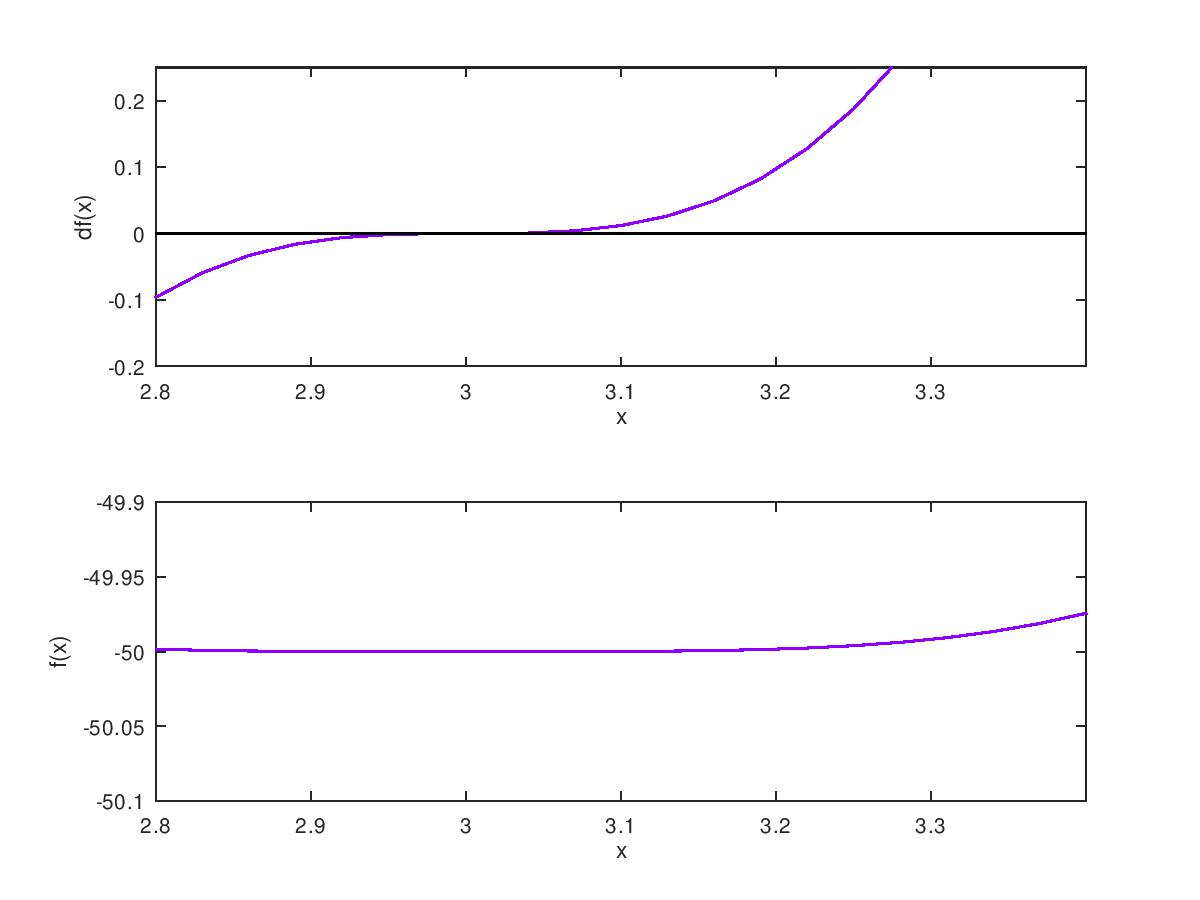
\includegraphics[scale=0.4]{0Bolcanoitter.jpg}
        \caption{инициализация}
    \end{figure}
    \begin{figure}[H]
        \centering
        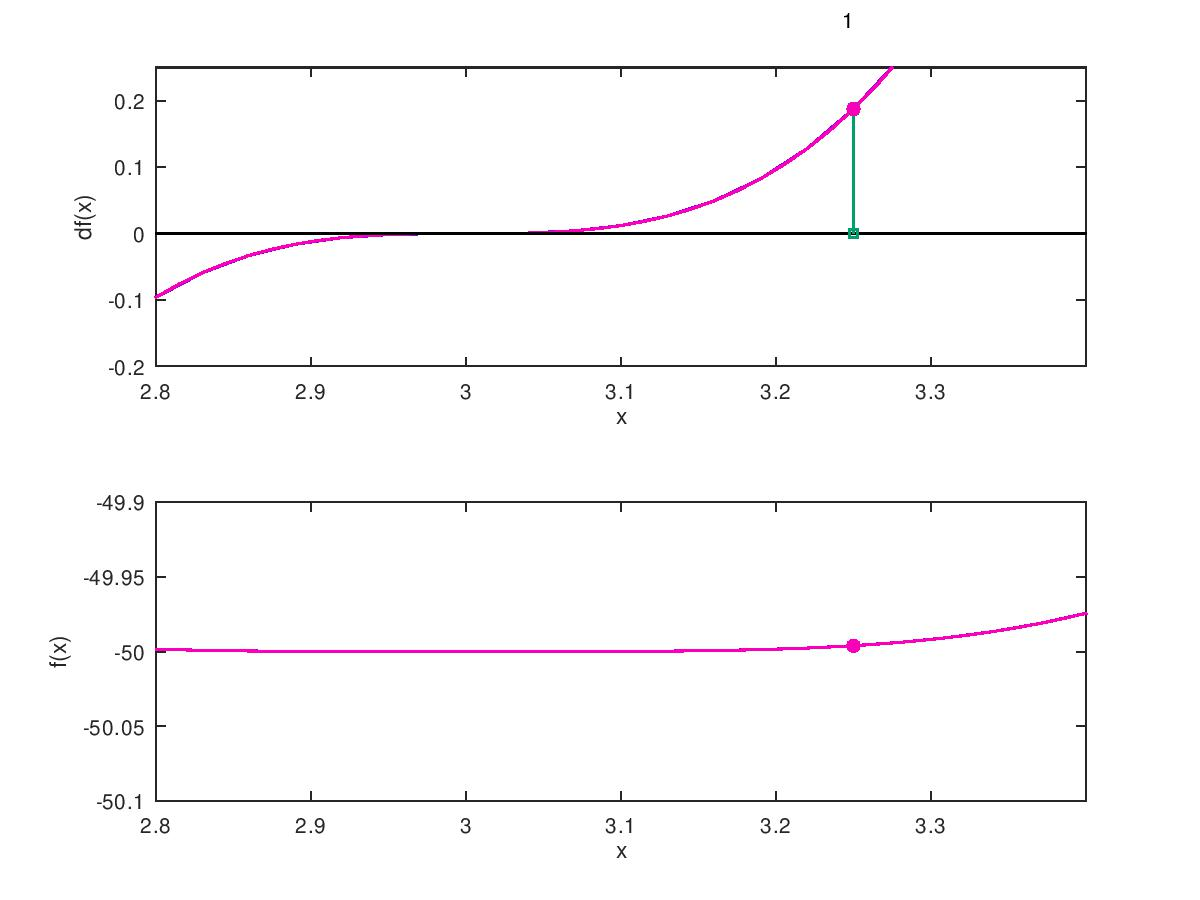
\includegraphics[scale=0.4]{1Bolcanoitter.jpg}
        \caption{Первая иттерация}
    \end{figure}
    \begin{figure}[H]
        \centering
        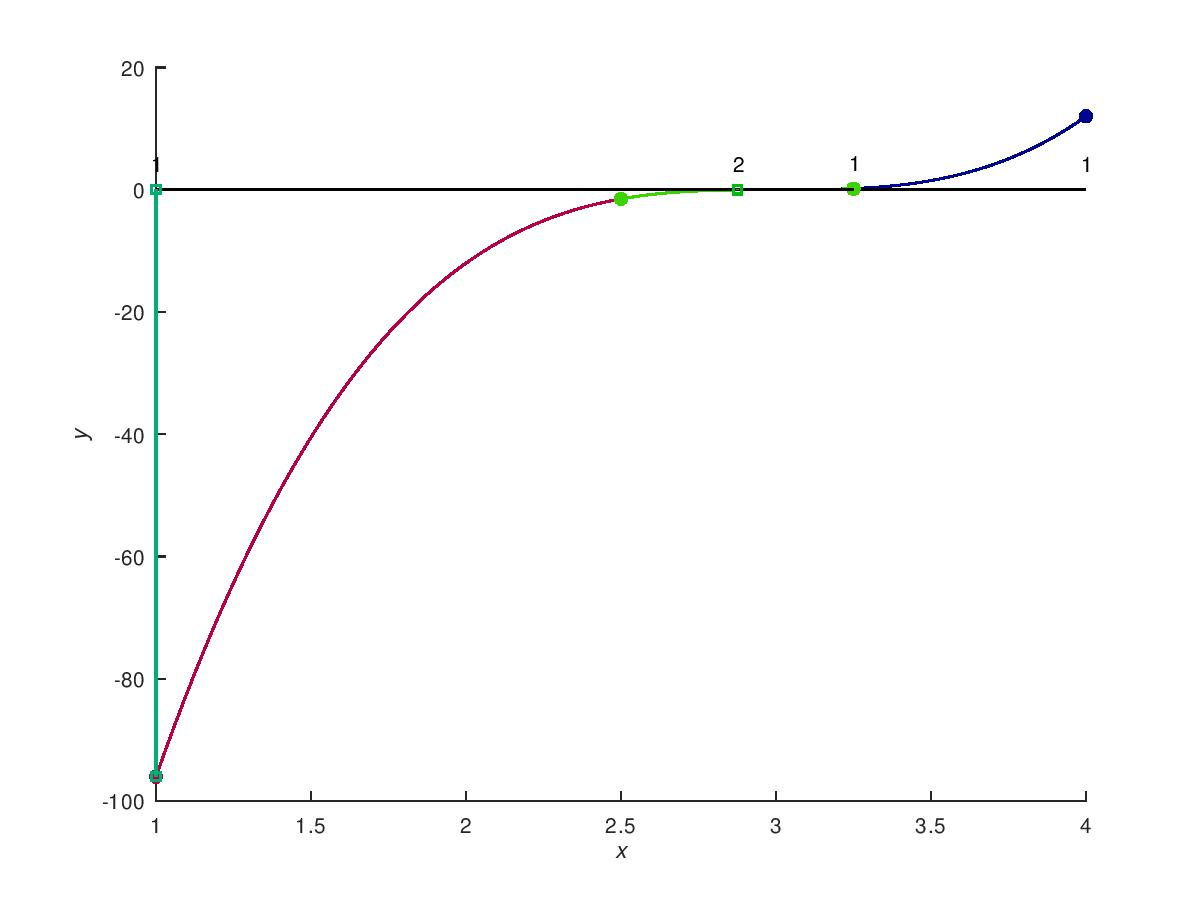
\includegraphics[scale=0.4]{2Bolcanoitter.jpg}
        \caption{Вторая иттерация}
    \end{figure}
    \begin{figure}[H]
        \centering
        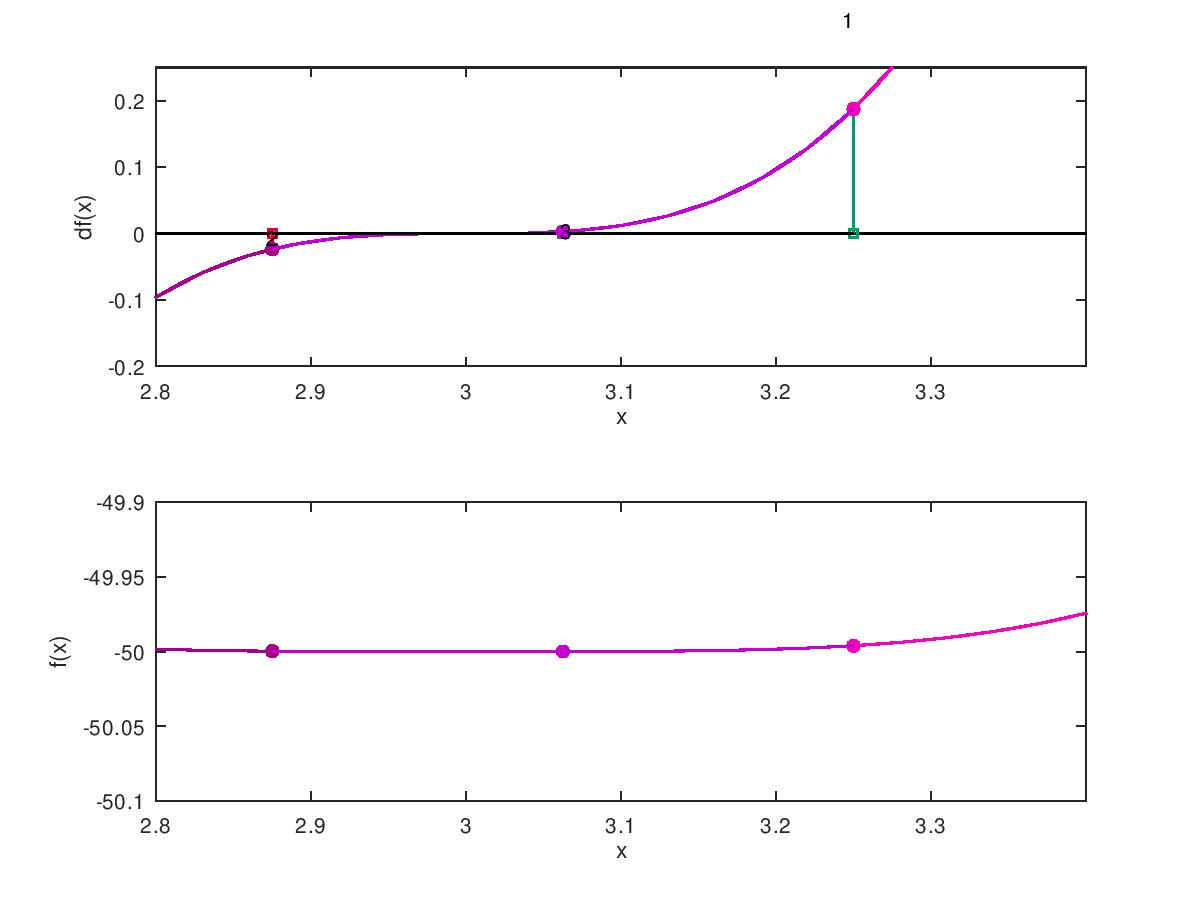
\includegraphics[scale=0.4]{3Bolcanoitter.jpg}
        \caption{Третья иттерация}
    \end{figure}
\newpage
\subsection*{Код метода секущих}
\begin{lstlisting}[style=Matlab-editor, caption=Метод секущих]

function [xk, k] = secant(dfunction, funct, a, b, tol)
    epsilon = tol;
    
    %Visualization
    ctr = 1;
    deltaX = (b-a) / 100;
    figure(3); hold on
    [miny, maxy] = drawplot(funct,a,b,a,b);
    deltaY = abs(maxy - miny)/100;
    placelabel(a,0,deltaX,deltaY,ctr);
    placelabel(b,0,deltaX,deltaY,ctr);
    
    %Main algorithm
    while 1
        xk = b - dfunction(b)*(b - a) / (dfunction(b) - dfunction(a))
        if dfunction(xk) <= epsilon
            break
        else
            if dfunction(xk) > 0
                b = xk
            else
                a = xk
            end
        end
        drawplot(funct,a,b,xk,xk);
        k = k + 1
    end
end

function [miny maxy] = drawplot(f,a,b,x1,x2)
    figure(3); 
    h = (b-a)/100;
    x = a:h:b;
    y = feval(f,x);
    
    miny = min(y);
    maxy = max(y);
    
    colp = hsv2rgb([rand(), 1, 0.5+0.5*rand()]);
    plot(x,y,'LineWidth',1,'Color',colp);
    scatter([a b],[feval(f,a), feval(f,b)],'Marker','o','MarkerFaceColor',colp,'MarkerEdgeColor',colp);
    xlabel('\itx');
    ylabel('\ity');
    line([a b],[0 0],'Color','k','LineWidth',1); %axis x
    col = hsv2rgb([rand(), 1, 0.5+0.5*rand()]);
    y1 = feval(f, x1);
    line([x1 x1],[0 y1],'Marker','s','Color',col,'LineWidth',1,'MarkerSize',4); 
    y2 = feval(f,x2);
    line([x2 x2],[0 y2],'Marker','s','Color',col,'LineWidth',1,'MarkerSize',4); 
    input("");
end

function placelabel(x,y,deltaX,deltaY,iternumber)
    if iternumber <=10
        text(x - deltaX/2, y + 4*deltaY, num2str(iternumber));
    end
end

\end{lstlisting}

\subsection*{Графики, демонстрирующие работу метода секущих}
    \begin{figure}[H]
        \centering
        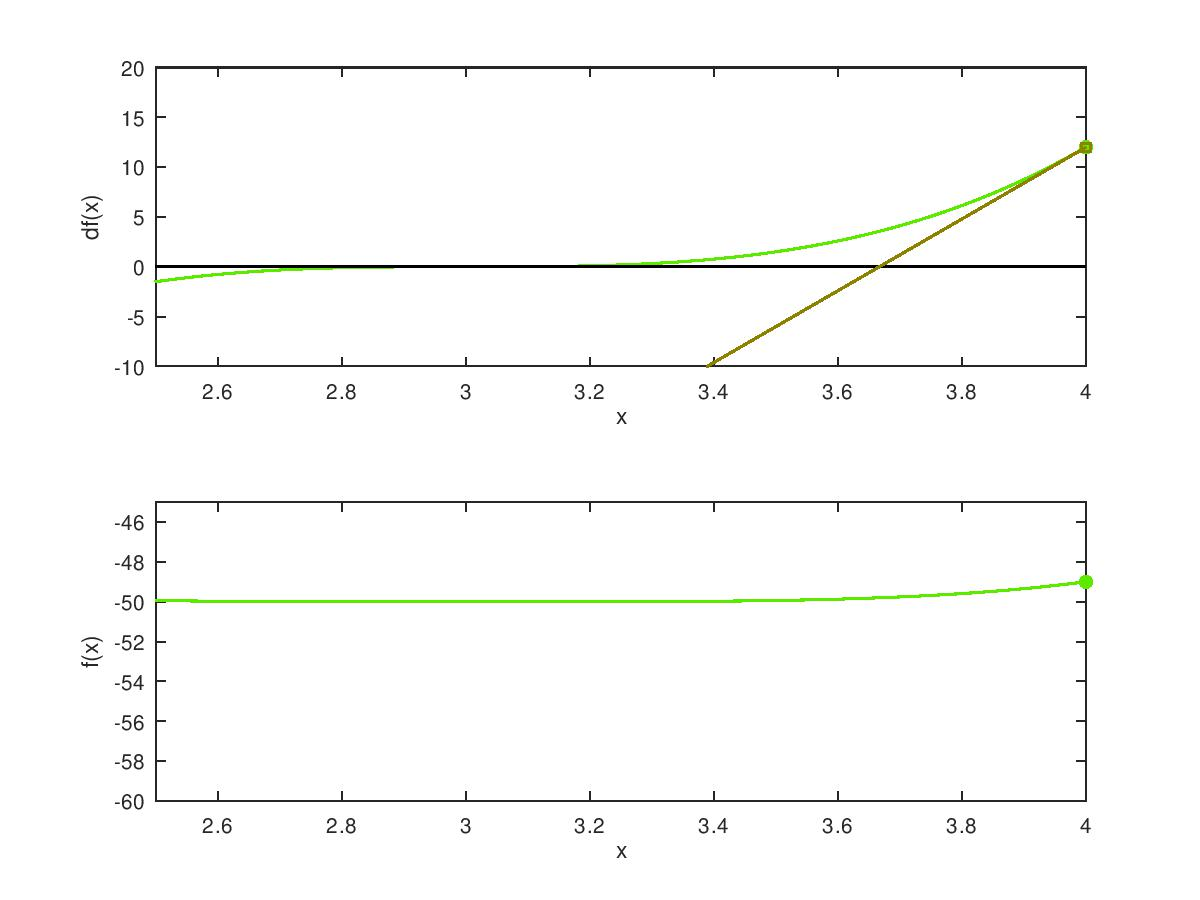
\includegraphics[scale=0.4]{0secantitter.jpg}
        \caption{инициализация}
    \end{figure}
    \begin{figure}[H]
        \centering
        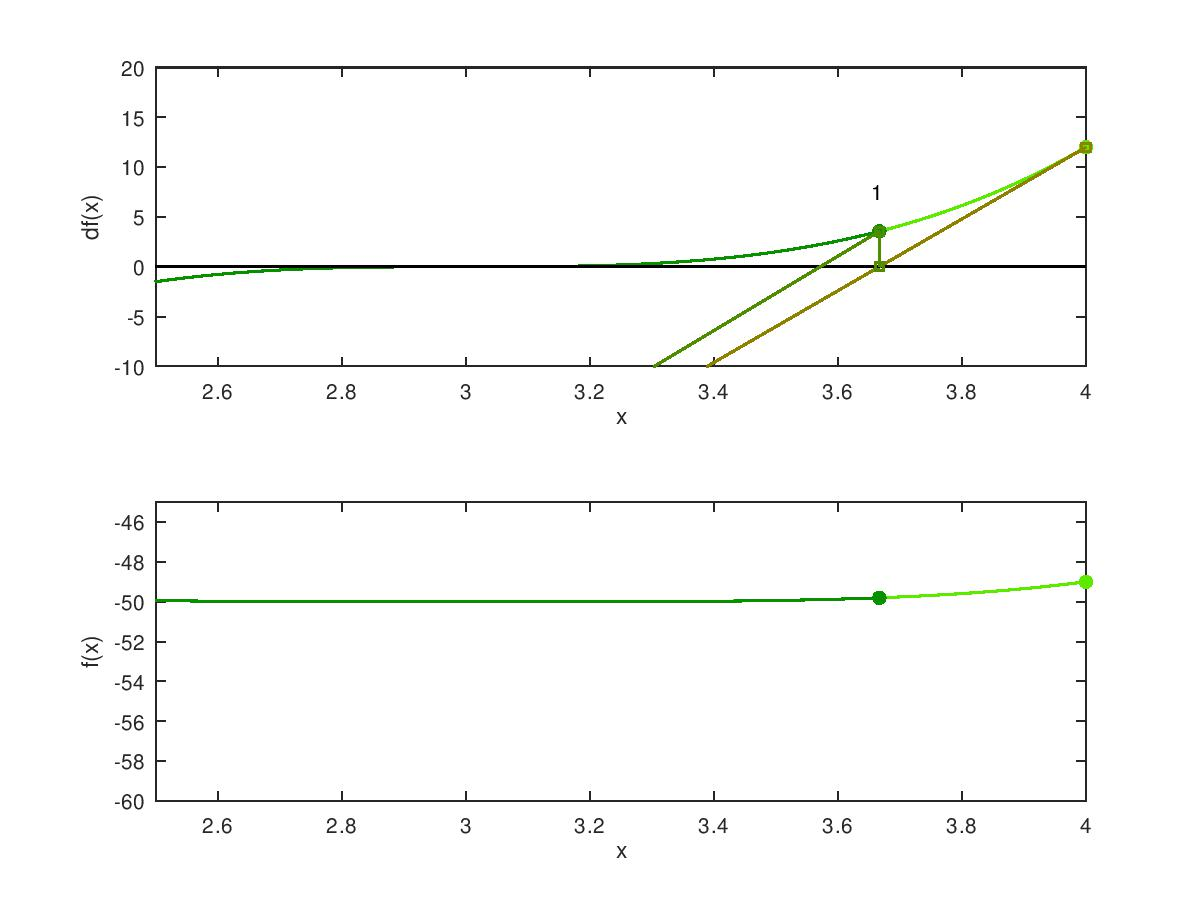
\includegraphics[scale=0.4]{1secantitter.jpg}
        \caption{Первая иттерация}
    \end{figure}
    \begin{figure}[H]
        \centering
        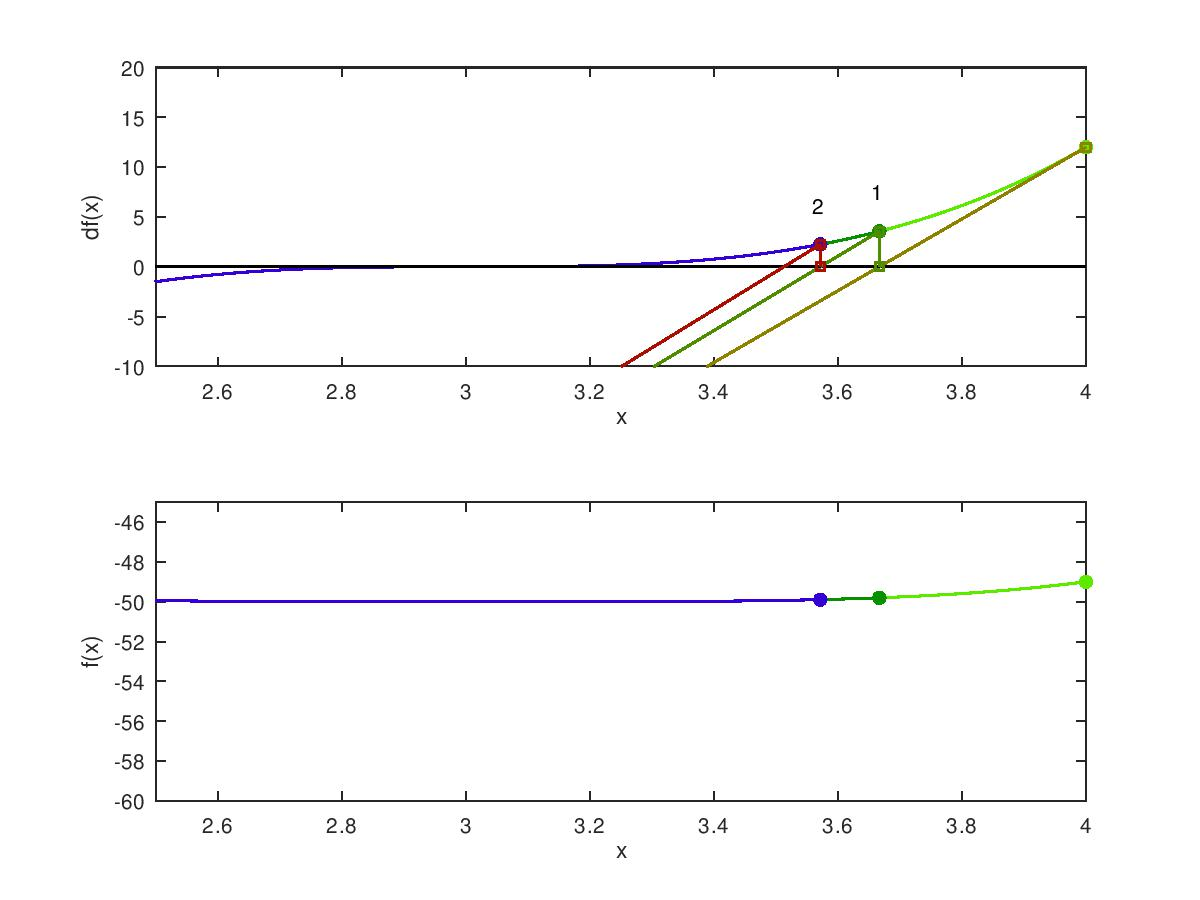
\includegraphics[scale=0.4]{2secantitter.jpg}
        \caption{Вторая иттерация}
    \end{figure}
    \begin{figure}[H]
        \centering
        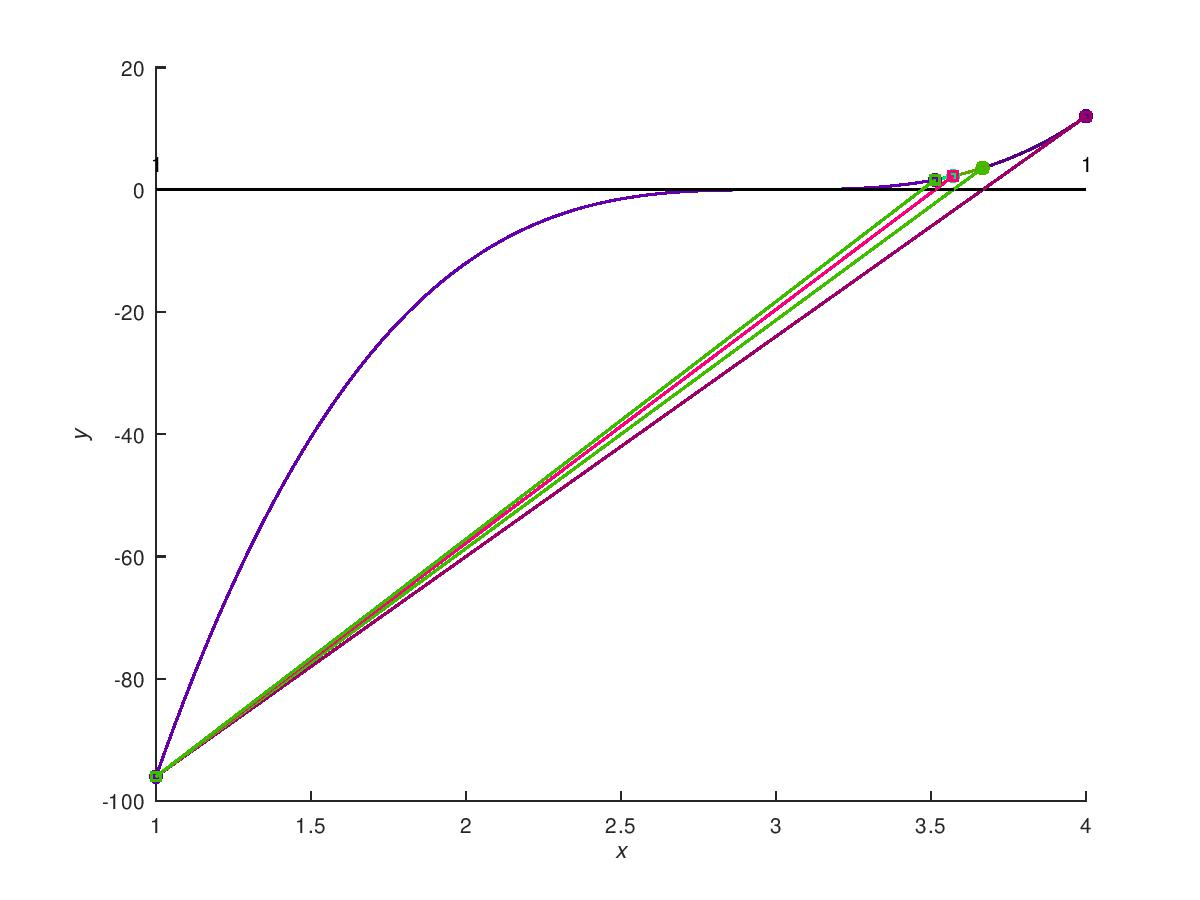
\includegraphics[scale=0.4]{3secantitter.jpg}
        \caption{Третья иттерация}
    \end{figure}
    \begin{figure}[H]
        \centering
        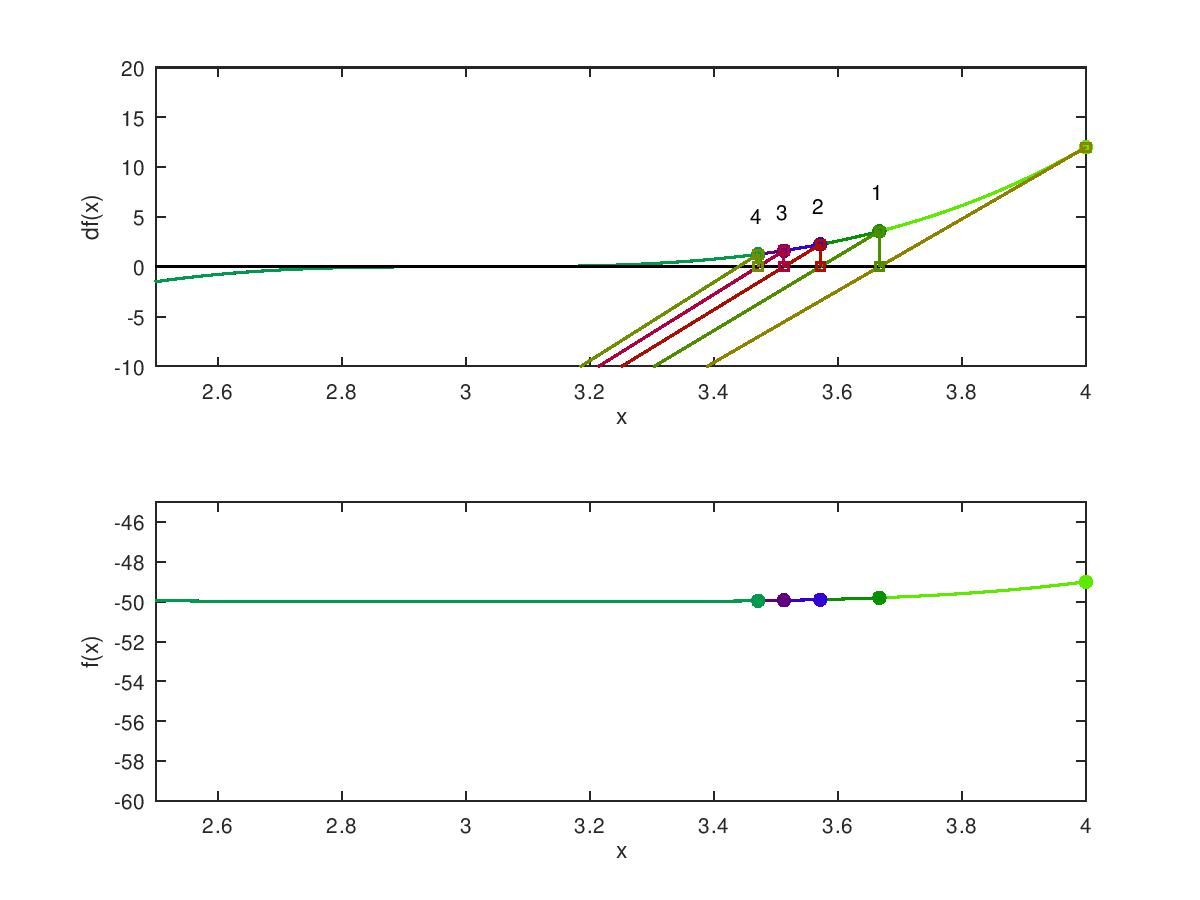
\includegraphics[scale=0.4]{4secantitter.jpg}
        \caption{Четвёртая иттерация}
    \end{figure}
    \begin{figure}[H]
        \centering
        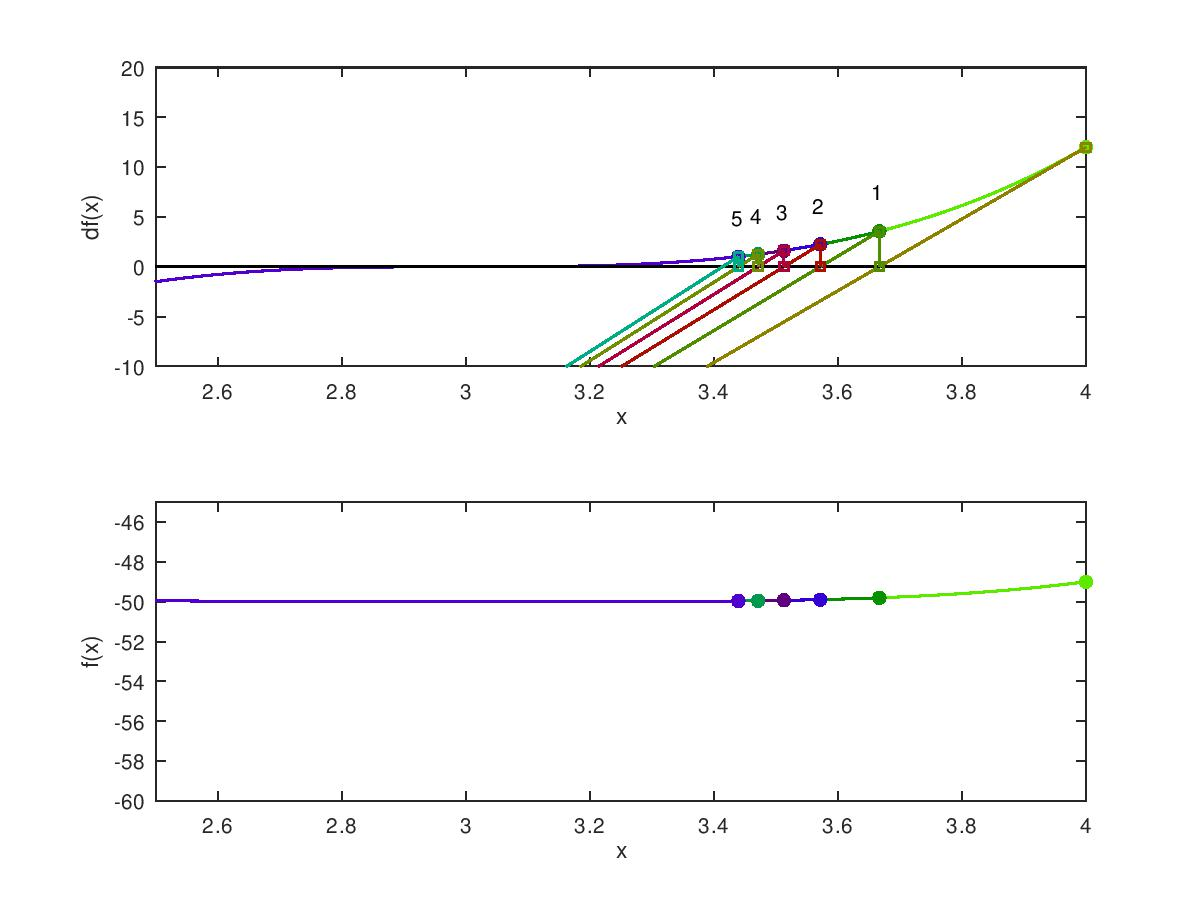
\includegraphics[scale=0.4]{5secantitter.jpg}
        \caption{Пятая иттерация}
    \end{figure}
    \begin{figure}[H]
        \centering
        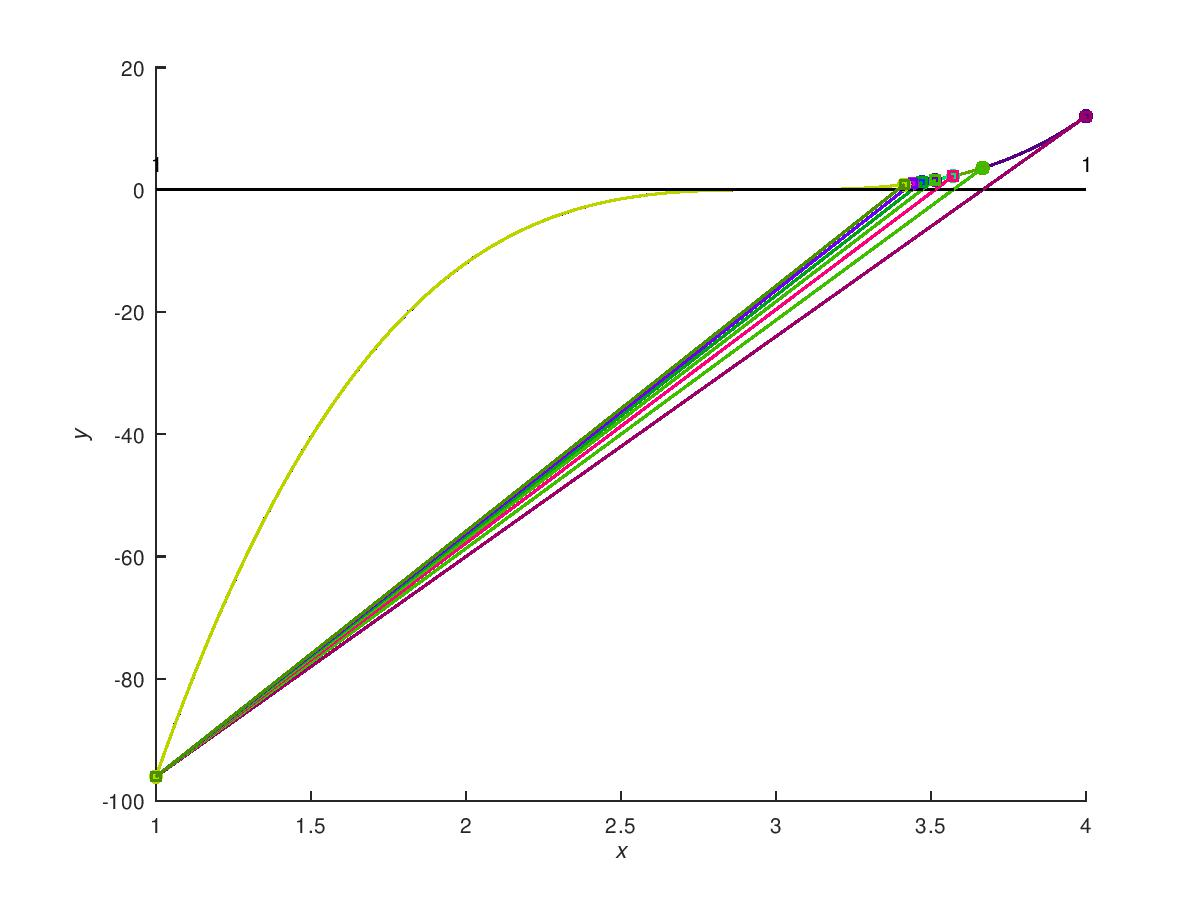
\includegraphics[scale=0.4]{6secantitter.jpg}
        \caption{Шестая иттерация}
    \end{figure}
    \begin{figure}[H]
        \centering
        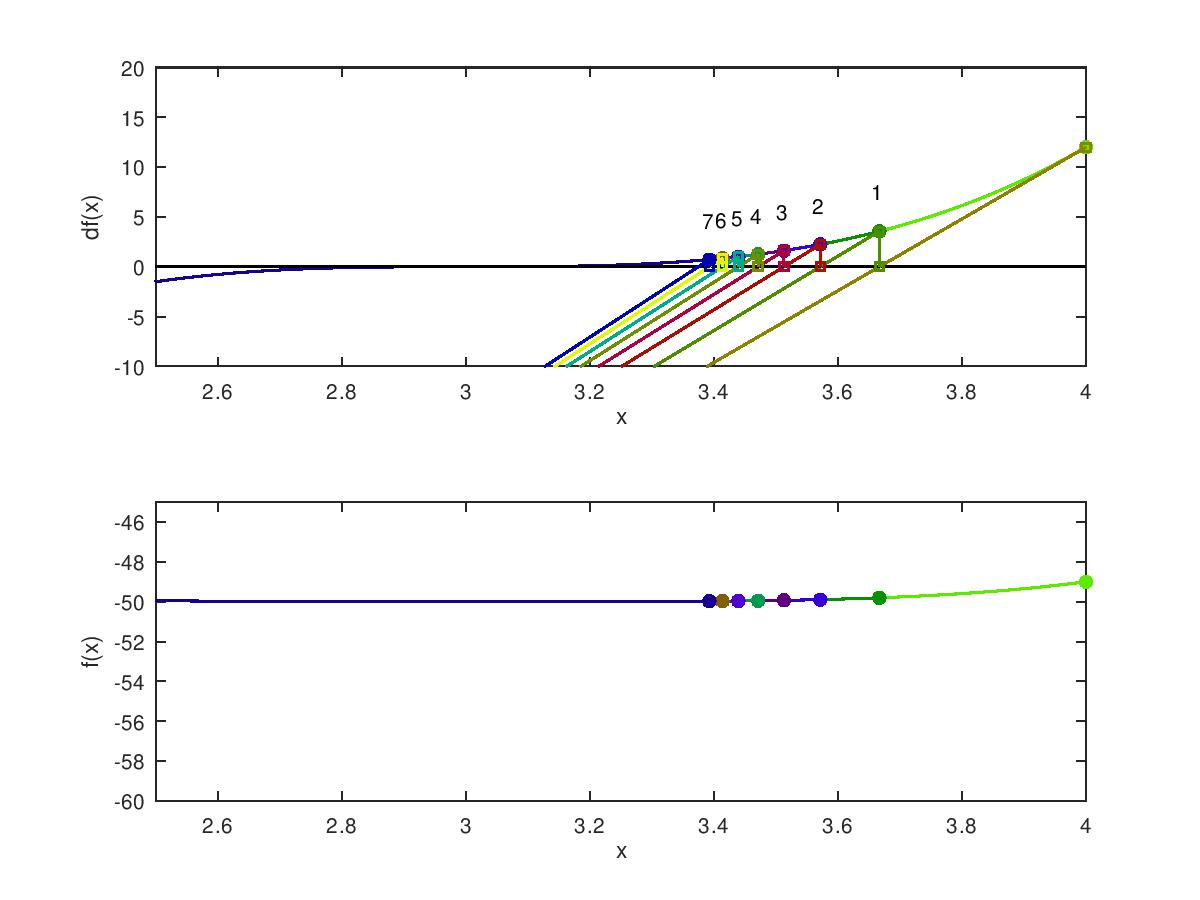
\includegraphics[scale=0.4]{7secantitter.jpg}
        \caption{Седьмая иттерация}
    \end{figure}
    \begin{figure}[H]
        \centering
        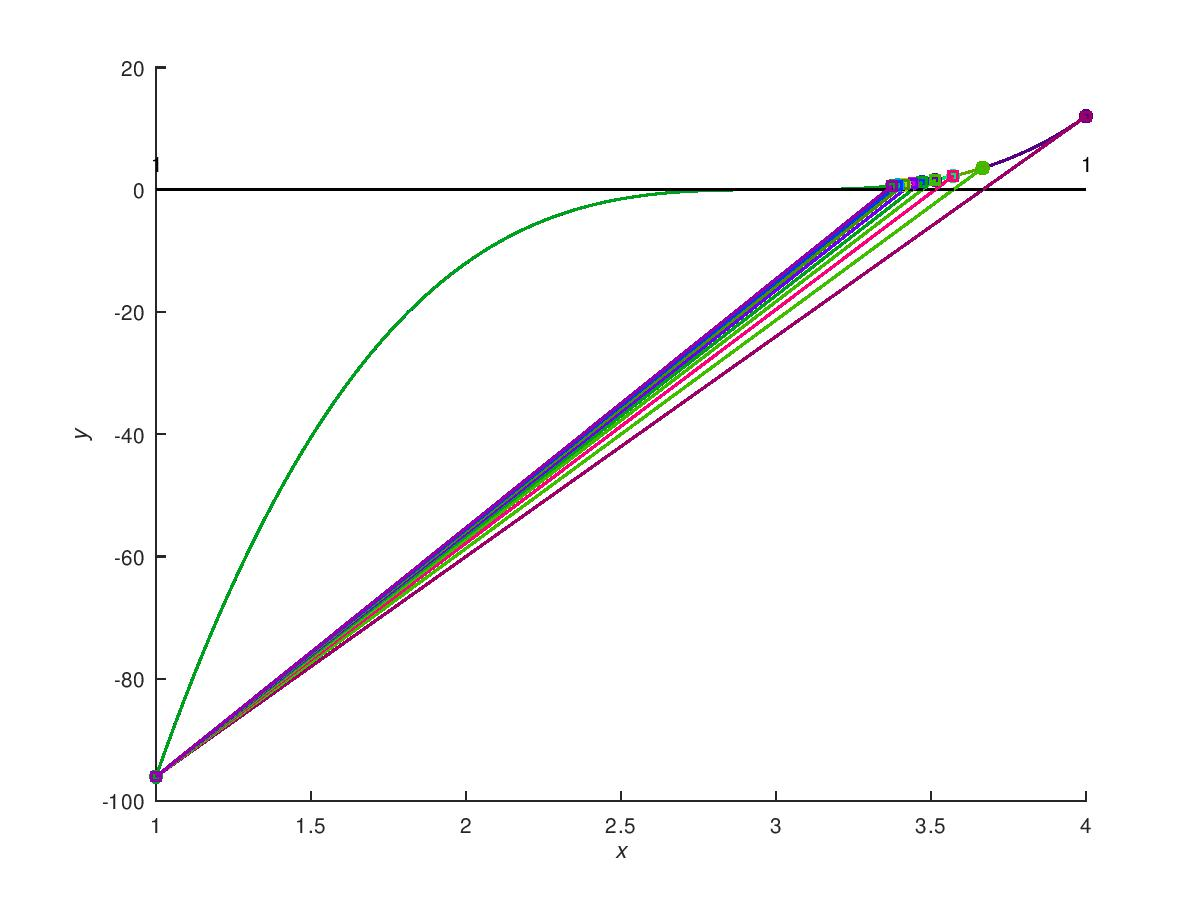
\includegraphics[scale=0.4]{8secantitter.jpg}
        \caption{Восьмая иттерация}
    \end{figure}
    \begin{figure}[H]
        \centering
        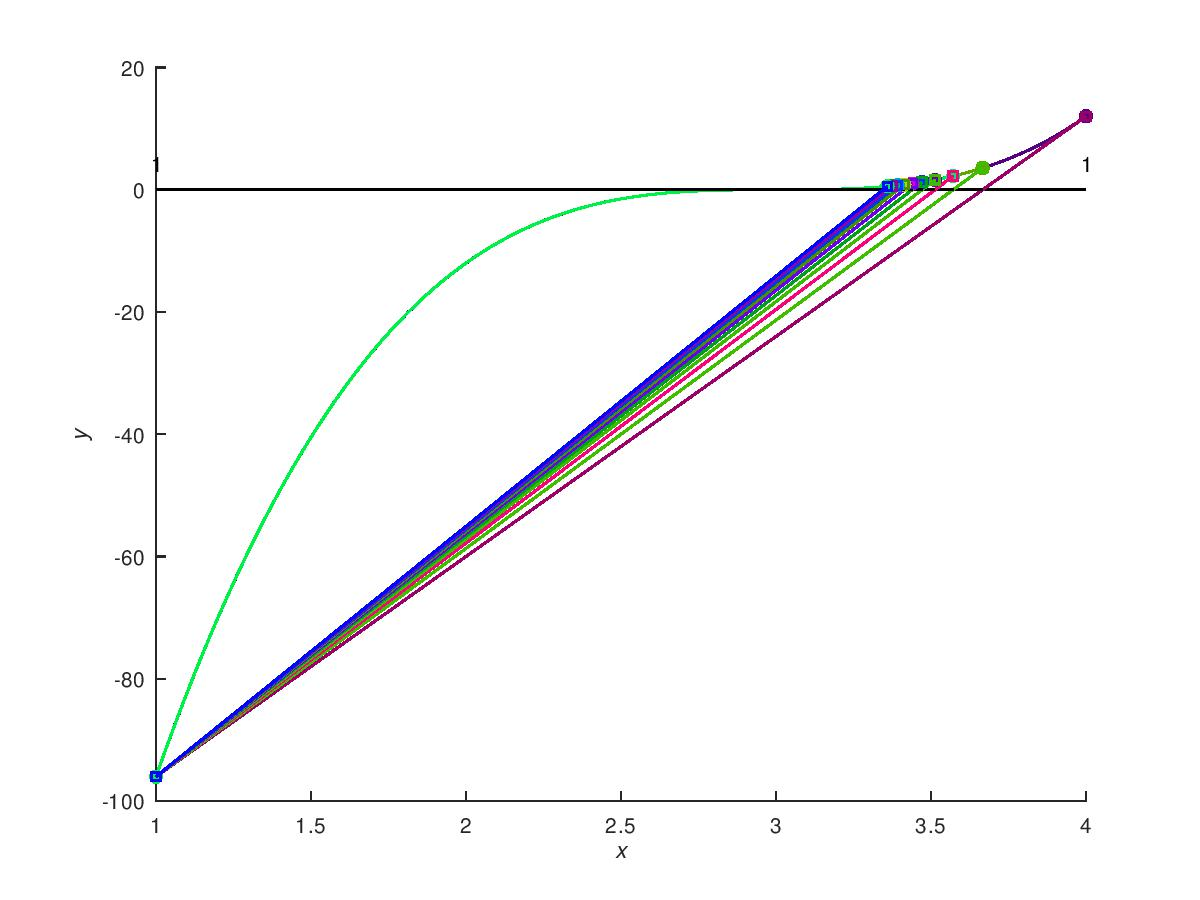
\includegraphics[scale=0.4]{9secantitter.jpg}
        \caption{Девятая иттерация}
    \end{figure}
\newpage    

%Здесь дожен быть график
\end{document}
